% PRIOR -----------------------------------
\section{Prior for DUMs}
\label{sec:prior}

In this section, we study the effect that the prior component has in DUMs. More specifically, we investigate the relationships between aleatoric uncertainty and the prior specified for DUMs. In particular, this is motivated by \citet{kapoor2022prior_cpe} which shows that using priors that forces model to be confident on the training data points can improve its performance by explicitly accounting for aleatoric uncertainty.
To this end, we look at \textit{entropy regularization} defining a training prior in the loss, \textit{prior evidence} and \textit{kernel function} defining a functional prior in the uncertainty head.

\textbf{Prior.} We compare different prior specifications including \textit{entropy regularization} defining a training prior in the loss, \textit{prior evidence} and \textit{kernel function} defining a functional prior in the uncertainty head. Entropy regularization is the entropy term $H(Q)$ in the Bayesian loss used to train NatPN which encourages a (uniform) prior distributions with high entropy \citep{charpentier2022natpn}. We control the strength of the regularization factor $\lambda$. Further, NatPN also explicitly defines a prior via the parameters $\chi^{prior}$ and $n^{prior}$. While  $\chi^{prior}$ defines the default categorical prediction via a uniform categorical distribution, the evidence parameter $n^{prior}$ defines the prior number of pseudo-observations and can be varied. Finally, we vary the prior of DUE by using different kernel functions in the learned GP including Matern kernel, RQ kernel, and RBF \citep{rasmussen2006gp}. \underline{\textit{Observation:}} Contrary to other Bayesian neural networks \citep{kapoor2022prior_cpe}, we observe that predictive and uncertainty performances of DUMs are not very sensitive to the prior specification (see \cref{fig:prior_ood,fig:prior_ood_brier,tab:kernel}), thus suggesting a higher robustness to prior mispecification. Nonetheless, a too strong entropy regularization toward an uniform prior degrades more performance of DUMs trained on dataset with low label noise than on high label noise. This suggests that a too high discrepancy between the model prior and the dataset aleatoric uncertainties can impact performance.

\begin{figure}[!htb]
    \centering
    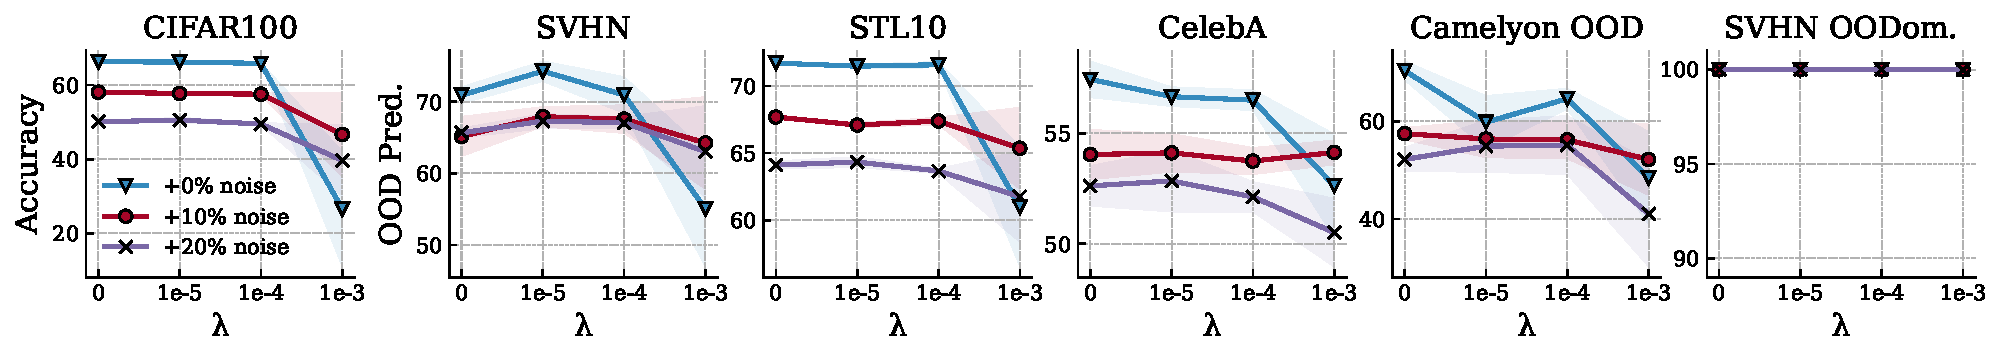
\includegraphics[width=\textwidth]{sections/008_iclr2023/figures/prior_entropy_acc_pred.pdf}
    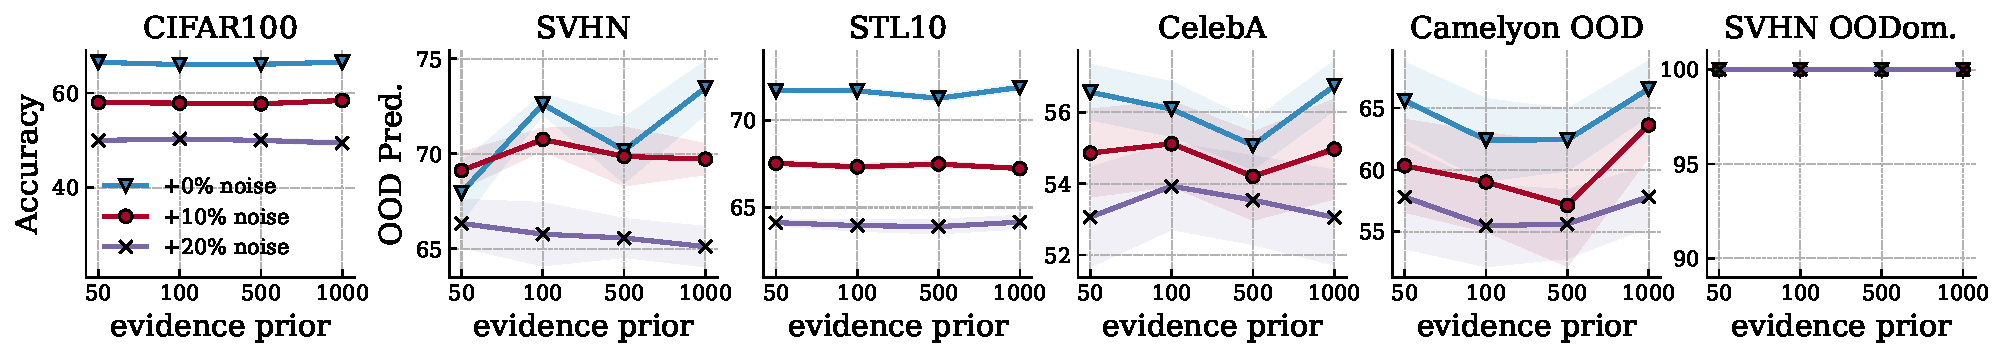
\includegraphics[width=\textwidth]{sections/008_iclr2023/figures/prior_pseudo_acc_pred.pdf}
    
    \caption{Results of enforcing different \textbf{prior} in NatPN on CIFAR100 by changing the (top) \textit{entropy regularization} $\lambda$ and the (bottom) \textit{evidence prior} $n^{prior}$. Different priors do not lead consistent results improvements.}
    \label{fig:prior_ood}
\end{figure}
 \vspace{-3mm}
\begin{table}[!htp]\centering
\caption{Results of enforcing different \textbf{prior} in DUE on CIFAR100 and Camelyon by changing the kernel function. OOD results are averaged over OOD datasets. Different priors lead to similar performance. }
\label{tab:kernel}
\vspace{-0mm}
\tiny
\resizebox{0.9\textwidth}{!}{%
\begin{tabular}{lcccccc}\toprule
&\multicolumn{3}{c}{\textbf{CIFAR100}} &\multicolumn{3}{c}{\textbf{Camelyon}} \\
\cmidrule(lr){2-4}\cmidrule(lr){5-7}
\textbf{Kernel} &\textbf{Accuracy ($\uparrow$)} &\textbf{Brier Score ($\downarrow$)} &\textbf{OOD Pred. ($\uparrow$)} &\textbf{Accuracy ($\uparrow$)} &\textbf{Brier Score ($\downarrow$)} &\textbf{OOD Pred. ($\uparrow$)} \\
\midrule
Matern52 &71.80 $\pm$ 0.18 &41.37 $\pm$ 0.24 &75.90 $\pm$ 1.18 &79.81 $\pm$ 2.72 &32.46 $\pm$ 3.22 &58.86 $\pm$ 6.20 \\
Matern32 &71.80 $\pm$ 0.21 &41.62 $\pm$ 0.22 &\textbf{76.15 $\pm$ 1.18} &80.23 $\pm$ 2.71 &32.77 $\pm$ 3.20 &58.50 $\pm$ 5.83 \\
Matern12 &71.70 $\pm$ 0.18 &43.10 $\pm$ 0.22 &75.70 $\pm$ 1.19 &79.30 $\pm$ 2.96 &32.67 $\pm$ 3.28 &\textbf{59.13 $\pm$ 6.39} \\
RQ &71.83 $\pm$ 0.19 &\textbf{41.16 $\pm$ 0.25} &75.93 $\pm$ 1.21 &80.31 $\pm$ 2.55 &32.22 $\pm$ 3.14 &58.69 $\pm$ 6.09 \\
RBF &\textbf{71.85 $\pm$ 0.19} &41.17 $\pm$ 0.24 &76.14 $\pm$ 1.19 &\textbf{80.45 $\pm$ 2.49} &\textbf{32.13 $\pm$ 3.11} &58.86 $\pm$ 5.91 \\
\bottomrule
\end{tabular}
}
\vspace{-3mm}
\end{table}


% \begin{table}[!htp]\centering
% \caption{\textbf{Uncertainty Head Prior.} (top) NatPN with a more expressive uncertainty head obtain significantly better performance. (bottom) DUE changing its uncertainty headoesn't have much effects. The reported OOD results are an average over all the independent OOD dataset result.}
% \label{tab:kernel}
% \tiny
% \begin{tabular}{lccccccccc}\toprule
% &\multicolumn{4}{c}{\textbf{CIFAR100}} &\multicolumn{4}{c}{\textbf{Camelyon}} \\
% \cmidrule(lr){2-5}\cmidrule(lr){6-9}
% \textbf{Head} &\textbf{Accuracy} &\textbf{Brier score} &\textbf{OOD Pred.} &\textbf{OOD Epis.} &\textbf{Accuracy} &\textbf{Brier score} &\textbf{OOD Pred.} &\textbf{OOD Epis.} \\
% \midrule
% Radial &71.09 $\pm$ 0.21 &52.27 $\pm$ 0.28 &72.84 $\pm$ 1.82 &50.95 $\pm$ 2.16 &83.14 $\pm$ 0.93 &24.55 $\pm$ 1.91 &60.27 $\pm$ 5.29 &69.16 $\pm$ 7.94 \\
% \textbf{NSF-R} &\textbf{71.61 $\pm$ 0.07} &\textbf{43.44 $\pm$ 0.11} &\textbf{73.54 $\pm$ 1.69} &\textbf{72.85 $\pm$ 1.25} &\textbf{89.84 $\pm$ 7.93} &\textbf{12.52 $\pm$ 6.17} &\textbf{64.14 $\pm$ 10.42} &\textbf{81.33 $\pm$ 8.78} \\

% \midrule
% \midrule

% Matern52 &71.80 $\pm$ 0.18 &41.37 $\pm$ 0.24 &75.90 $\pm$ 1.18 &- &79.81 $\pm$ 2.72 &32.46 $\pm$ 3.22 &58.86 $\pm$ 6.20 &- \\
% Matern32 &71.80 $\pm$ 0.21 &41.62 $\pm$ 0.22 &\textbf{76.15 $\pm$ 1.18} &- &80.23 $\pm$ 2.71 &32.77 $\pm$ 3.20 &58.50 $\pm$ 5.83 &- \\
% Matern12 &71.70 $\pm$ 0.18 &43.10 $\pm$ 0.22 &75.70 $\pm$ 1.19 &- &79.30 $\pm$ 2.96 &32.67 $\pm$ 3.28 &\textbf{59.13 $\pm$ 6.39} &- \\
% RQ &71.83 $\pm$ 0.19 &\textbf{41.16 $\pm$ 0.25} &75.93 $\pm$ 1.21 &- &80.31 $\pm$ 2.55 &32.22 $\pm$ 3.14 &58.69 $\pm$ 6.09 &- \\
% RBF &\textbf{71.85 $\pm$ 0.19} &41.17 $\pm$ 0.24 &76.14 $\pm$ 1.19 &- &\textbf{80.45 $\pm$ 2.49} &\textbf{32.13 $\pm$ 3.11} &58.86 $\pm$ 5.91 &- \\
% \bottomrule
% \end{tabular}
% \end{table}